\normaltrue
\correctiontrue

%\UPSTIidClasse{11} % 11 sup, 12 spé
%\newcommand{\UPSTIidClasse}{12}

\exer{Mouvement RT  $\star$ \label{C1:05:05}}
\setcounter{question}{0}\UPSTIcompetence[2]{B2-14}
\UPSTIcompetence[2]{B2-15}
\UPSTIcompetence[2]{C1-05}
\index{Compétence B2-14}
\index{Compétence B2-15}
\index{Compétence C1-05}
\index{Torseur des actions mécaniques transmissibles}
\index{Torseur d’une action mécanique extérieure}
\index{Principe fondamental de la statique}
\index{PFS}
\index{Mécanisme à 1 rotation et 1 translation}
\ifcorrection
\else
\marginnote{\textbf{Pas de corrigé pour cet exercice.}}
\fi

\ifprof
\else
Soit le mécanisme suivant. On a $\vect{AB}=\lambda(t)\vect{i_1}$ et $\vect{AC}=R\vect{i_1}$. De plus :
\begin{itemize}
\item $G_1$ désigne le centre d'inertie de \textbf{1} et $\vect{AG_1}=L_1\vect{i_1}$, on note $m_1$ la masse de \textbf{1}; %et $\inertie{G_1}{1}=\matinertie{A_1}{B_1}{C_1}{0}{0}{0}{\bas{1}}$; 
\item $G_2=B$ désigne le centre d'inertie de \textbf{2}, on note $m_2$ la masse de \textbf{2}.% et $\inertie{G_2}{2}=\matinertie{A_2}{B_2}{C_2}{0}{0}{0}{\bas{2}}$.
\end{itemize}


Un moteur électrique positionné entre \textbf{0} et \textbf{1} permet de maintenir \textbf{1} en équilibre.
Un vérin électrique positionné entre \textbf{1} et \textbf{2} permet de maintenir \textbf{2} en équilibre.

L'accélération de la pesanteur est donnée par $\vect{g}=-g\vect{j_0}$.

\begin{center}
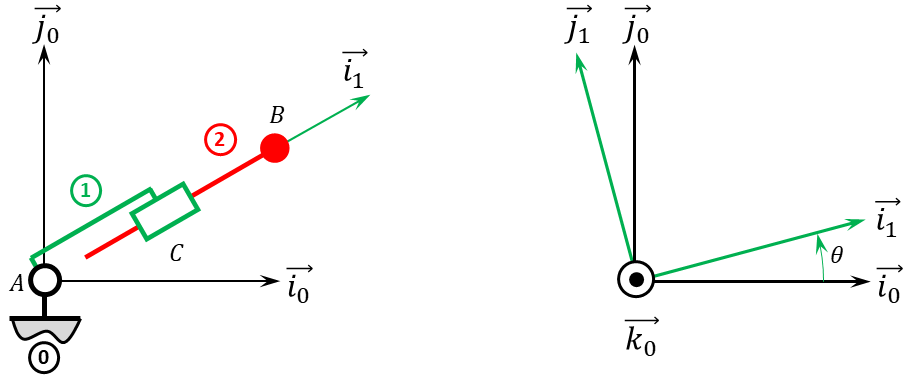
\includegraphics[width=\linewidth]{05_RT_01_bis}
\end{center}
\fi

\question{Réaliser le graphe d'analyse en faisant apparaître l'ensemble des actions mécaniques.}
\ifprof
\begin{center}
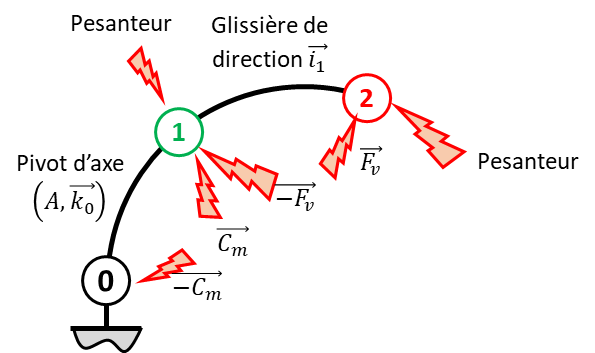
\includegraphics[width=\linewidth]{05_RT_01_cor}
\end{center}

\else
\fi

\question{Donner le torseur de chacune des actions mécaniques.}
\ifprof
\begin{itemize}
\item liaison glissière : $\torseurstat{T}{1}{2} = \torseurl{Y_{12}\vj{1}+Z_{12}\vk{1}}{L_{12}\vi{1}+M_{12}\vj{1}+N_{12}\vk{1}}{C}$;
%tel que $\vectf{1}{2}\cdot\vi{1} = 0$;
\item pesanteur sur 2 : $\torseurstat{T}{\text{pes}}{2} = \torseurl{-m_2 g \vj{0}}{\vect{0}}{B}$;
 %avec $-m_2 g \vj{0} \cdot \vi{1} = -m_2 g\sin \theta$;
\item action du vérin $\torseurstat{T}{\text{Vérin}}{2} =  \torseurl{F_v \vi{1}}{\vect{0}}{A}$.
\item liaison pivot : $\torseurstat{T}{0}{1}= \torseurl{X_{01}\vi{1}+Y_{01}\vj{1}+Z_{01}\vk{1}}{L_{01}\vi{1}+M_{01}\vj{1}}{C}$;
% tel que $\vectm{A}{0}{1}\cdot\vk{0} = 0$.
%\item pesanteur sur 2 : $\torseurstat{T}{\text{pes}}{2} = \torseurl{-m_2 g \vj{0}}{\vect{0}}{B}$
% avec $\vectm{A}{\text{pes}}{2} \cdot \vk{0} = \left(\vect{AB}\wedge -m_2 g \vj{0} \right)\cdot \vk{0}$
%$= \left(\lambda(t) \vi{1} \wedge -m_2 g \vj{0} \right)\cdot \vk{0}$
%$= -m_2 g\lambda(t)\cos\theta(t) $;
\item pesanteur sur 1 : $\torseurstat{T}{\text{pes}}{1} = \torseurl{-m_1 g \vj{0}}{\vect{0}}{G_1}$;
% avec $\vectm{A}{\text{pes}}{1} \cdot \vk{0} = \left(\vect{AG_1}\wedge -m_1 g \vj{0} \right)\cdot \vk{0}$
%$= \left(L_1 \vi{1}\wedge -m_1 g \vj{0} \right)\cdot \vk{0}$
%$= -m_1 gL_1\cos\theta(t) $;
\item action du moteur $\torseurstat{T}{\text{Moteur}}{1} =  \torseurl{\vect{0}}{C_m \vk{0}}{A}$.
\end{itemize}

\else
\fi

\question{Simplifier les torseurs dans l'hypothèse des problèmes plans.}
\ifprof
\begin{itemize}
\item liaison glissière : $\torseurstat{T}{1}{2} = \torseurl{Y_{12}\vj{1}}{N_{12}\vk{1}}{C}$;
\item pesanteur sur 2 : $\torseurstat{T}{\text{pes}}{2} = \torseurl{-m_2 g \vj{0}}{\vect{0}}{B}$;
\item action du vérin $\torseurstat{T}{\text{Vérin}}{2} =  \torseurl{F_v \vi{1}}{\vect{0}}{A}$.
\item liaison pivot : $\torseurstat{T}{0}{1}= \torseurl{X_{01}\vi{1}+Y_{01}\vj{1}}{\vect{0}}{C}$;
\item pesanteur sur 1 : $\torseurstat{T}{\text{pes}}{1} = \torseurl{-m_1 g \vj{0}}{\vect{0}}{G_1}$;
\item action du moteur $\torseurstat{T}{\text{Moteur}}{1} =  \torseurl{\vect{0}}{C_m \vk{0}}{A}$.
\end{itemize}

\else
\fi

\question{Proposer une démarche permettant de déterminer le couple et l'effort que doivent développer chacun des actionneurs  pour maintenir le mécanisme en équilibre.}
\ifprof

\begin{itemize}
\item On isole \textbf{\{1\}}. On réalise un théorème de la résultante statique en projection sur $\vect{i_1}$ :
$ \vectf{1}{2}\cdot \vect{i_1} + \vectf{F_v}{2}\cdot \vect{i_1} + \vectf{\text{Pes}}{2}\cdot \vect{i_1} = 0$.
\item On isole \textbf{\{1+2\}}. On réalise un théorème du moment statique en $A$ en projection sur $\vect{k_0}$ :
$ \vectm{A}{0}{1}\cdot \vect{k_0} 
+ \vectm{A}{\text{Mot}}{1}\cdot \vect{k_0} 
+ \vectm{A}{\text{Pes}}{2}\cdot \vect{k_0}
+ \vectm{A}{\text{Pes}}{1}\cdot \vect{k_0} = 0$.
\end{itemize}

\else
\fi


\question{Proposer une démarche permettant de déterminer les efforts inconnus dans les liaisons.}
\ifprof

\begin{itemize}
\item On isole \textbf{\{1\}}. On réalise un théorème de la résultante statique en projection sur $\vect{j_1}$ 
et un théorème du moment statique $C$ en projection sur $\vect{k_1}$ .
\item On isole \textbf{\{1+2\}}. On réalise un théorème de la résultante statique en projection sur $\vect{i_1}$ et $\vect{j_1}$.
\end{itemize}
\else
\fi

\ifprof
\else
\begin{flushright}
\footnotesize{Corrigé  voir \ref{C1:05:05}.}
\end{flushright}%
\fi